\documentclass{article}
\usepackage[utf8]{inputenc}
\usepackage{tikz}
\usepackage{float}
\usepackage{amsmath}
\usepackage[numbers]{natbib}
\usepackage{todonotes}
\usepackage{bm}
\usepackage{setspace}
\usepackage{subcaption}
\usepackage{caption}
\usepackage{textcomp}
\captionsetup{font=footnotesize}
\usepackage[margin=.8in]{geometry}
\usepackage{algorithm}
\usepackage{algpseudocode}
\usepackage{url}
% Thing Dave added these
\usepackage{amssymb}
\usepackage{amsthm}
\newtheorem{theorem}{Theorem}
\usepackage{changes}
\usetikzlibrary{arrows,positioning}

\newcommand{\Unif}{\text{Unif}}
\newcommand{\Beta}{\text{Beta}}
\newcommand{\Normal}{\text{Normal}}
\newcommand{\Binomial}{\text{Binomial}}
\newcommand{\E}{\mathbb{E}}
 \doublespacing
\title{}
\author{Graham Casey Gibson, Dan Sheldon, Evan Ray, Nicholas Reich }

\begin{document}


\maketitle

\section{Introduction}
COVID-19 has become a worldwide pandemic that has effected all continents, causing over 308,000 cases and 13,000 deaths. The viral agent (SARS-CoV-2) is extremely contagious with an estimate of $R_0$ between $2.5$ and $3.5$. \cite{https://github.com/midas-network/COVID-19/tree/master/parameter_estimates/2019_novel_coronavirus} With the arrival of the virus in the U.S., significant effort has been made to model the spread of the disease.

We see this effort as having two distinct endpoints. The first is to model the number of COVID-19 cases in the population and the second is to model the effects of COVID-19 on influenza surveillance networks such as ILInet. Since 2015, the CDC has been running an influenza-like-illness (defined by fever >100 and cough or sore throat, referred to as ILI) prediction initiative. The goal is to forecast the percent of patients who meet the symptomatic criteria, out of the patients who present to the network. Since the outbreak of COVID-19 in the U.S., efforts have shifted to harnessing influenza surveillance networks to monitor the pandemic. Because of the symptom overlap, it is expected that ILI will pick up COVID-19 cases without requiring a confirmed positive test. This as advantageous for two reasons, first, the network is already in place with a defined network of hospitals and providers reporting, and second, the lack of available testing means waiting for confirmed cases may delay an accurate estimate of the true number of cases. 

In this work, we consider two approaches to model the effects of COVID-19 on ILInet. 
\section{Explicit SIR Model}
\begin{center}
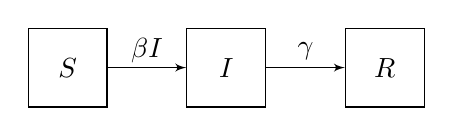
\begin{tikzpicture}[node distance=1cm,auto,>=latex',every node/.append style={align=center},int/.style={draw, minimum size=1cm}]
    \node [int] (S)             {$S$};
    \node [int, right=of S] (I) {$I$};
     \node [int, right=of I] (R) {$R$};

    \coordinate[right=of I] (out);
    \path[->, auto=false] (S) edge node {$\beta I$ \\[.2em]} (I)
                          (I) edge node {$\gamma$       \\[.2em] } (out) ;
                          \end{tikzpicture}
\end{center}

Thanks to the efforts of JHU (\cite{https://www.google.com/url?q=https://github.com/CSSEGISandData/COVID-19/&sa=D&source=hangouts&ust=1584972954968000&usg=AFQjCNGnOaY2YaOoRx7GLJkyiEmNRlz7Aw}) we have available case counts in a time series for all 50 states. In particular, we have a time series of confirmed cases we call $C_{i,j}$ where $i$ indexes calendar time and $j$ indexes regions, in this case states. 

We can model the confirmed cases using the SIR model as 


\begin{equation}
  C_{i,j} \sim N(I_{i,j},\sigma^2) 
 \end{equation}
  
  \begin{equation}
\begin{bmatrix} S_{i,j} \\
   I_{i,j} \\
   R_{i,j} 
  \end{bmatrix}  
  =  f\left(
  \begin{bmatrix} S_{i-1,j} \\
   I_{i-1,j} \\
   R_{i-1,j} 
  \end{bmatrix}|\beta_j,\gamma_j \right)
\end{equation}

where $f$ is the RK4 approximation to the differential equation parameterized by $\beta,\gamma$. We use, 




$$
\begin{aligned}
I_0 &\sim \Unif(0, 0.02) \\
\gamma &\sim \Gamma(k_\gamma, k_\gamma \hat{d}) \\
\beta &\sim \Gamma(k_\beta, k_\beta \hat{d}/\hat{R}) \\
\rho &\sim \Beta(\kappa\hat{\rho}, \kappa(1-\hat{\rho}))\\
\end{aligned}
$$
?
These satisfy: $\E[\gamma] = 1/\hat{d}$, $\E[\beta] = \hat{R}/\hat{d}$, $\E[\rho] = \hat{\rho}$
?
The user-selected parameters and current values are:
\begin{itemize}
 \item $k_\gamma = k_\beta = 1$ shape parameters for $\gamma$, $\beta$
\item $\hat{d} = 10$ estimate of duration in infected compartment
\item $\hat{R} = 2.2$ estimate of $R_0$
\item  $\hat{\rho} = 0.3$ initial guess of detection rate
\item $\kappa = 50$ concentration parameter for detection rate
\end{itemize}

\subsection{Interventions}

Currently in progress. 

\subsection{Incorporating ILI}

In addition, we have the publicly available ILI data for the same calendar dates and regions, we call $\text{ILI}_{i,j}$. We consider this the sum of both non-COVID-19 case counts and COVID-19 case counts. That is 

\begin{equation}
\text{ILI}_{i,j} = \frac{\text{ILI}^{\text{non-COVID-19 cases}}_{i,j} + C_{i,j}}{\text{ILI}^{\text{patients}}_{i,j}}
\label{eq:1}
\end{equation}

We have well developed process models for $\frac{\text{ILI}^{\text{non-COVID-19 cases}}_{i,j} }{\text{ILI}^{\text{patients}}_{i,j}}$ that have been implemented in the FluSight challenge to predict ILI. However, we do not have well developed process models for $\text{ILI}^{\text{non-COVID-19 cases}}_{i,j}$ and $\text{ILI}^{\text{patients}}_{i,j}$ individually.  In order to use our existing process models for influenza driven ILI we re-write \eqref{eq:1} as 


\begin{equation}
\text{ILI}_{i,j} = \frac{\text{ILI}^{\text{non-COVID-19 cases}}_{i,j}}{\text{ILI}^{\text{patients}}_{i,j}} + \frac{C_{i,j}}{\text{ILI}^{\text{patients}}_{i,j}}
\label{eq:2}
\end{equation}

Equation \eqref{eq:2} allows us to use ILI process models to predict the first term. However, we still need to model $\text{ILI}^{\text{patients}}_{i,j}$ for the second term. 
This model defines the likelihood over observed $ILI_{i,j}$ and confirmed COVID-19 cases $C_{i,j}$ for a given time-point and region $j$ as:

\begin{equation}
\mathcal{L}(\text{ILI}_{i,j},C_{i,j} | \beta, \gamma,\text{ILI}_{1:(i-1),*},C_{1:(i-1),*}) = \mathcal{L}(\text{ILI}_{i,j} | \text{ILI}_{1:(i-1),*}) *\mathcal{L}(C_{i,j}  | \beta, \gamma,C_{1:(i-1),*})
\end{equation}

which is the product of the likelihood over the observed $ILI$ and the observed COVID-19 cases. 

\subsection{Confounding of ILI and COVID-19}

As of March 2020, we expect $ILI$ to be confounded between non-COVID-19 and COVID-19. That is, beyond this cutoff we do not observe $\text{ILI}^{\text{non-COVID-19 cases}}$ but rather, $\text{ILI}^{\text{non-COVID-19 cases}} + \text{ILI}^{\text{COVID-19 cases}}$. In order to directly model $\text{ILI}^{\text{non-COVID-19 cases}}$ we restrict the model to only use historical $ILI$ data before March of 2020. We therefore use a kernel density estimate of $ILI$ from historical seasons.

\section{Latent SIR Model}

A second option that avoid the complexity of modeling the expected number of patients who will present to the influenza surveillance network, is to treat the SIR curve as a latent variable without directly tying it to confirmed COVID-19 cases. 




\end{document}